\documentclass[]{ccs-thesis}
% options:
% [germanthesis] - Thesis is written in German
% [plainunnumbered] - Don't print numbers on plain pages
% [earlydraft] - Settings for quick draft printouts
% [watermark] - Print current time/date at bottom of each page
% [phdthesis] - switch to PhD thesis style
% [twoside] - double sided
% [cutmargins] - text body fills complete page

% Choose one of the following lines.
\group{Cooperative Mobile Systems}
%\group{Distributed Embedded Systems}

% Author name. Separate multiple authors with commas.
\author{Maximilian W. Gotthardt}
\birthday{13. July 1993}
\birthplace{Berlin}

% Title of your thesis.
\title{ESP-Now as light protocol for situational purposes}

% Choose one of the following lines, changing the word "Computer Science" to match your degree program.
\thesistype{Bachelor's Thesis in Computer Engeneering}\thesiscite{Bachelor's Thesis~(Bachelorarbeit)}
%\thesistype{Bachelor Thesis in Computer Science}\thesiscite{Bachelor Thesis~(Bachelorarbeit)}
%\thesistype{Seminar Thesis in Computer Science}\thesiscite{Seminar Thesis~(Seminararbeit)}

% List of advisors, separated by commas. Delete if identical to referees or inapplicable.
\advisors{Anatolij Zubow}

% List of referees, separated by commas.
\referees{TODO: List of referees}


% Define abbreviations used in the thesis here.
\acrodef{WSN}{Wireless Sensor Network}
\acrodef{MANET}{Mobile Ad Hoc Network}
\acrodef{ROI}{Region of Interest}{short-indefinite={an}, long-plural-form={Regions of Interest}}
\acrodef{ADAC}{German Automobile Association}{foreign={Allgemeiner Deutscher Automobilclub}}
\acrodef{CANhashing}[CAN]{Content Addressable Network}{extra={when referring to the distributed hash table}}
\acrodef{CANproto}[CAN]{Controller Area Network}{extra={when referring to the bus protocol}}

\begin{document}

\pagenumbering{roman}

\maketitle

\thispagestyle{empty}

\cleardoublepage

\TODO{This template is for use with \texttt{pdflatex} and \texttt{biber}. It has been tested with TeX~Live 2018 (as of 1 April 2019).}

\chapter*{Abstract}
\addcontentsline{toc}{chapter}{Abstract}
\begin{otherlanguage*}{american}

about 1/2 page:
\begin{enumerate}
	\item Motivation (Why do we care?)
	\item Problem statement (What problem are we trying to solve?)
	\item Approach (How did we go about it)
	\item Results (What's the answer?)
	\item Conclusion (What are the implications of the answer?)
\end{enumerate}

\end{otherlanguage*}


\chapter*{Kurzfassung}
\addcontentsline{toc}{chapter}{Kurzfassung}
\begin{otherlanguage*}{ngerman}

Gleicher Text (sinngemäß, nicht wörtlich) in Deutsch

\end{otherlanguage*}
\acresetall

\cleardoublepage
\tableofcontents
\TODO{The table of contents should fit on one page. When in doubt, adjust the \texttt{tocdepth} counter.}

\cleardoublepage
\pagenumbering{arabic}

\chapter{Guidelines}

The following are general guidelines for how to write a thesis, with a special focus on how to use the template we provide.
Please read it in full before starting.

This template already includes a large number of LaTeX packages.
Make sure you use an up-to-date LaTeX distribution, such as \emph{TeX Live 2017}.
Familiarize yourself with the available package options of this template (such as the \texttt{germanthesis} and \texttt{watermark} options).


\section{Typesetting}

You can include many non-ASCII characters (like umlauts äöü or accented characters in general ñçø) verbatim in your \texttt{.tex} code, but make sure to save the file using UTF-8 encoding.

Use double quotation marks only for text cited from other work ``like this''.
Use bold text \textbf{very sparingly}, as it is likely to interrupt a reader's flow of reading.
Instead, use the \texttt{emph} command to typeset such text in a \emph{somewhat} less intrusive way (while still indicating a change in the tone of voice).

Use paragraphs to break the content into logical groups.
Do not use hard\\ line breaks. In the source file, however, line breaks have proven to simplify editing considerably: putting exactly one sentence per line makes it very easy to move content around, it helps quickly identifying overly long sentences, and allows line-based diff tools to work as expected.

Consider using the \texttt{textsc} command to make long runs of capital letters slightly less intrusive.
Typesetting PCMCIAPEBKAC as \textsc{Pcmciapebkac} makes the text stand out much less on the page.


\section{Cross References}
\label{sec:cross-ref}

Cross references are an easy way to point a reader to certain parts of the text.
For figures, tables, and equations, they are a must.
Sometimes, it is also useful to point a reader to other sections, e.g., to \cref{sec:cross-ref}, but this should be used sparingly.

\section{Figures}

\begin{figure}%
	\centering
	\subfloat[coverage]{\label{fig:setup1}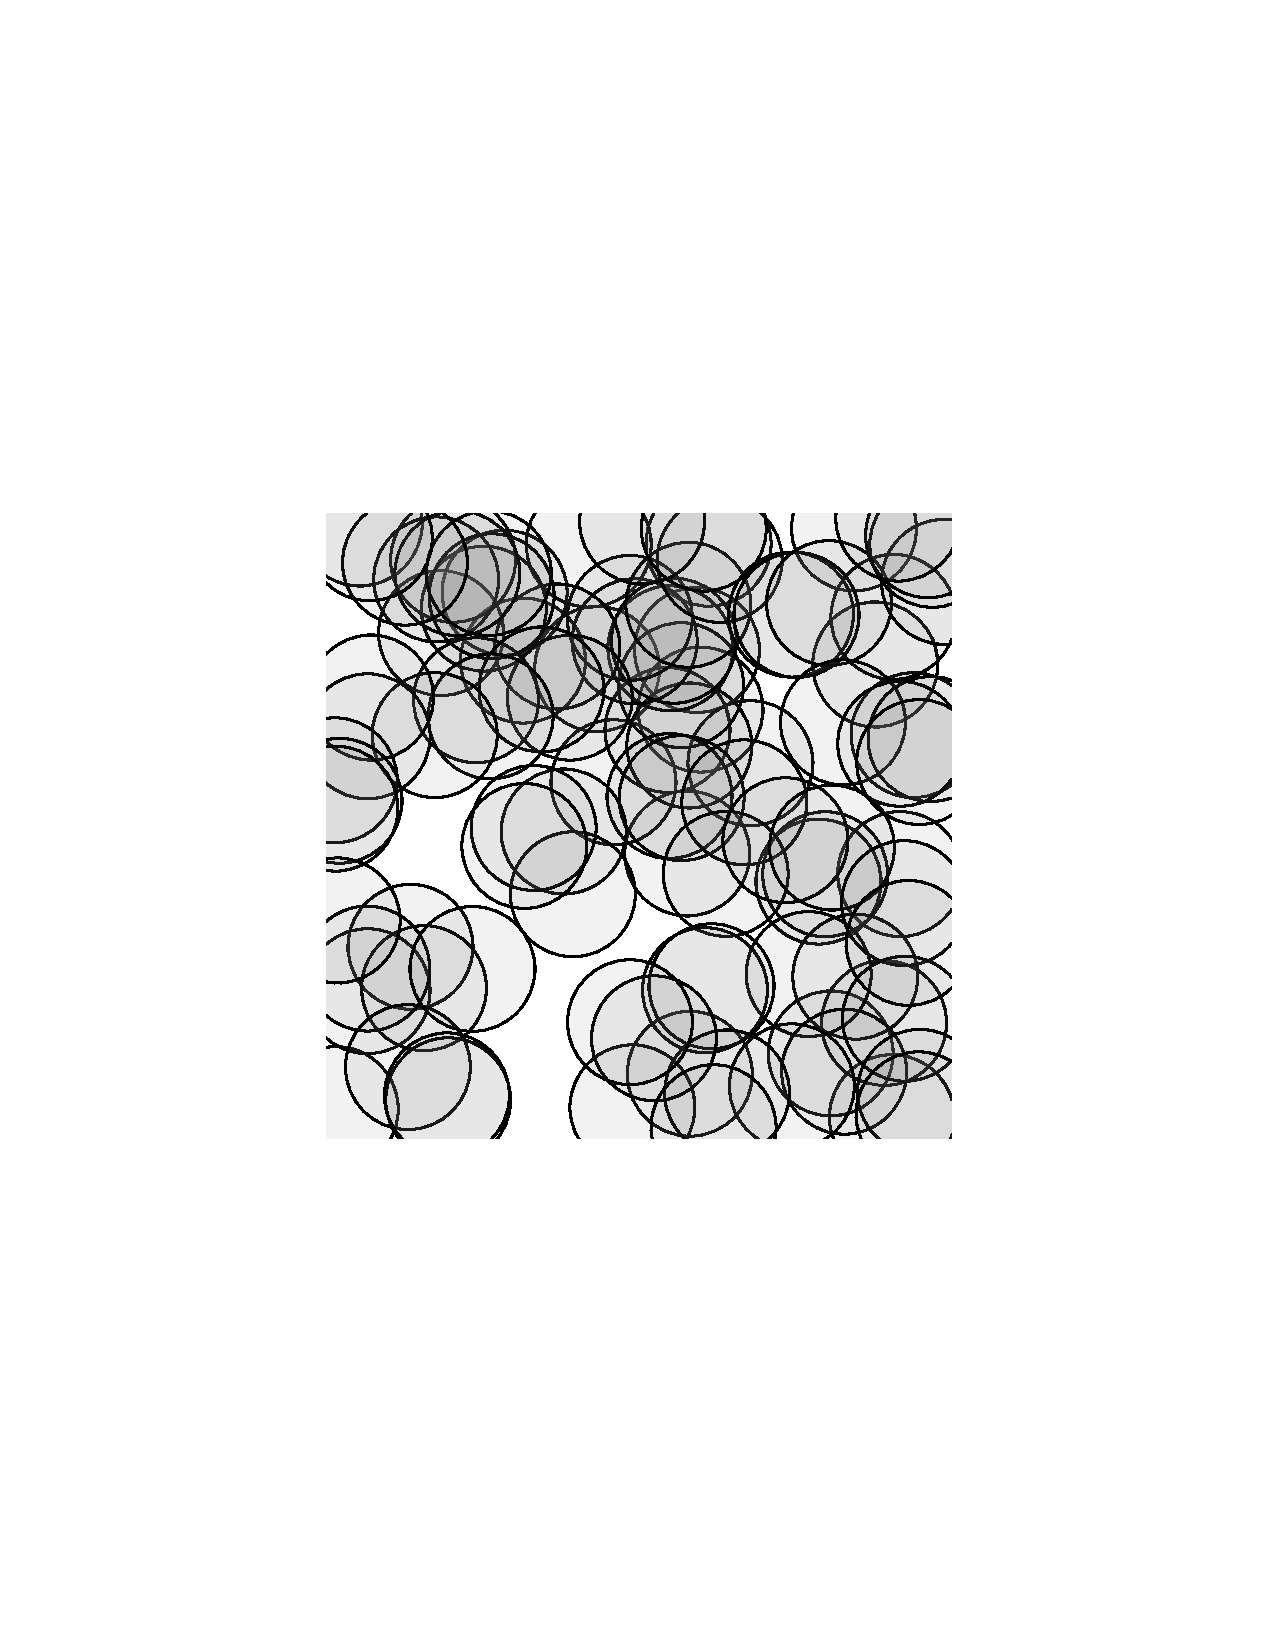
\includegraphics[width=0.3\textwidth]{figures/coverage-30--0-static1}}%
	\subfloat[connectivity]{\label{fig:setup2}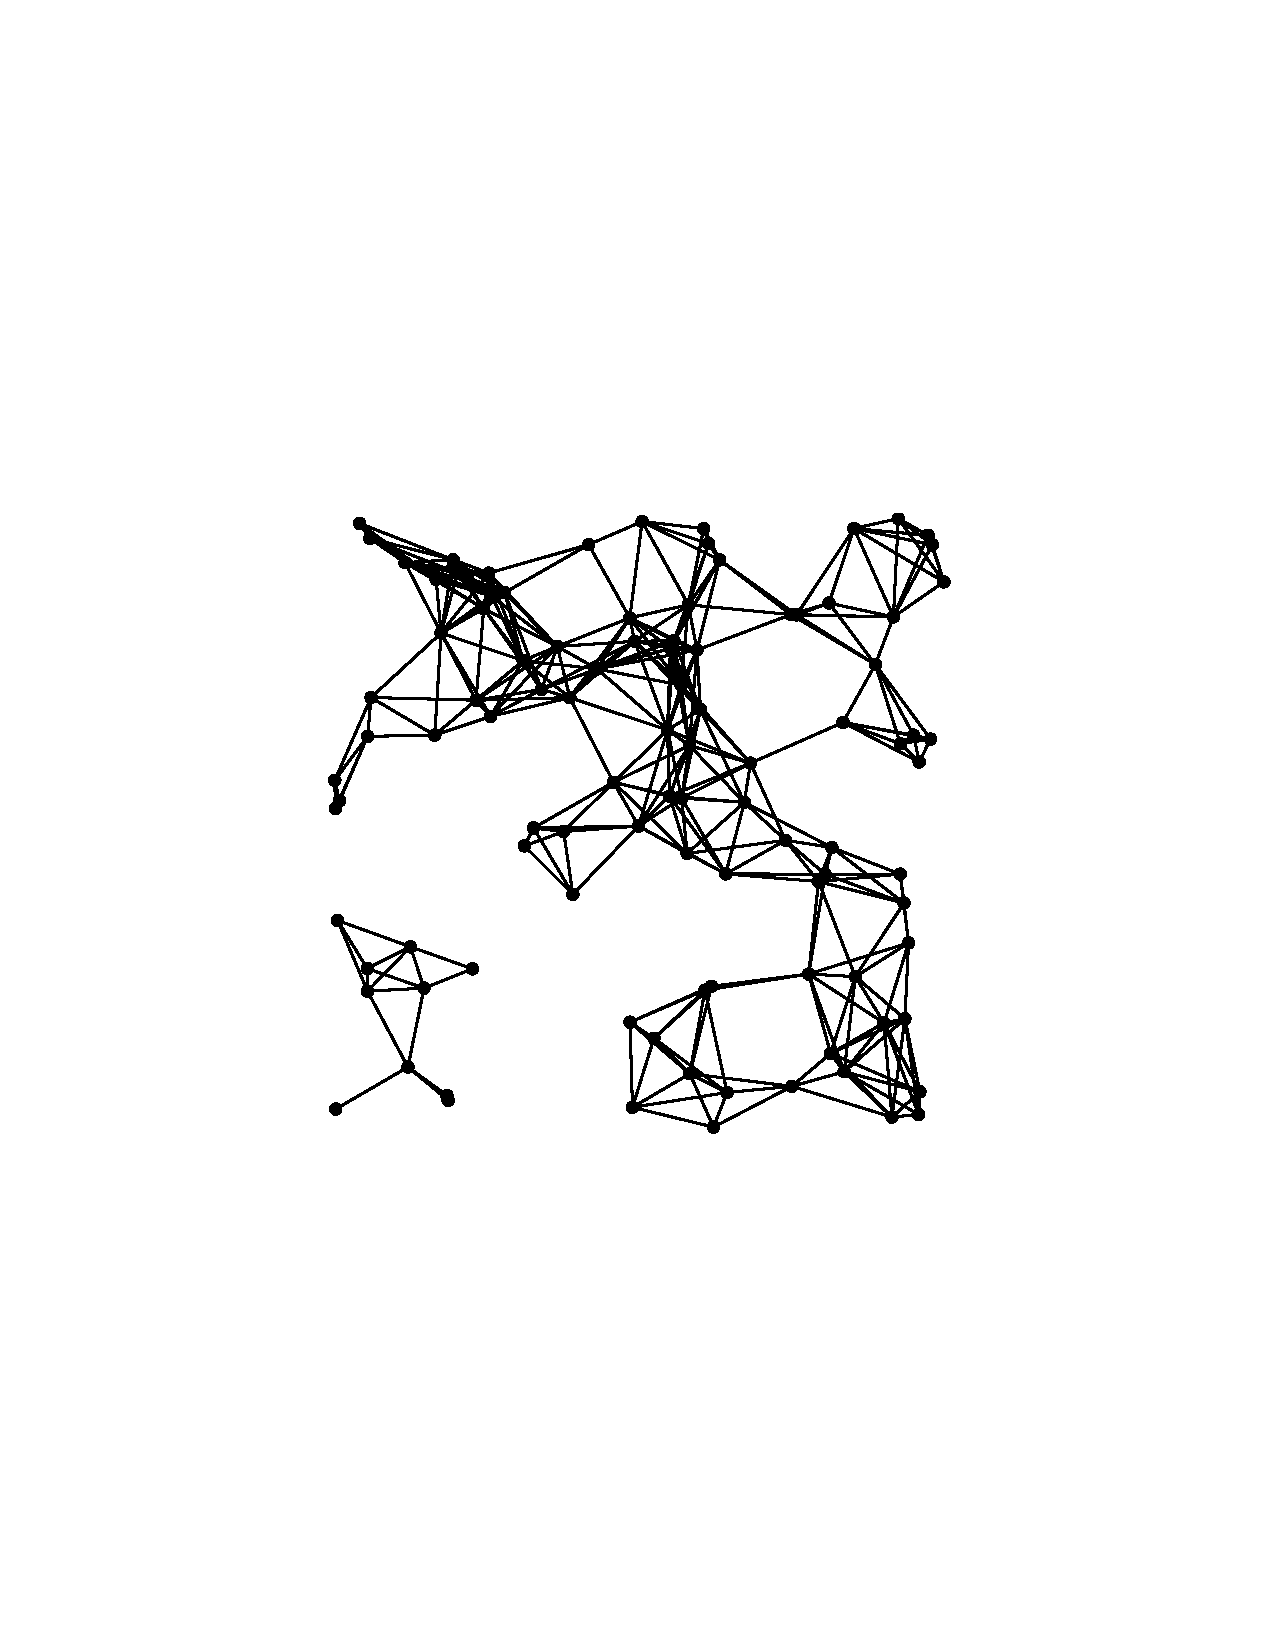
\includegraphics[width=0.3\textwidth]{figures/connectivity-50-0-static1}}
	\caption{Subfigures showing coverage and connectivity for a sample replication at time $t=0$}%
	\label{fig:setups12}%
\end{figure}

A picture says more than a thousand words.
Use \texttt{jpeg} files for photos, use \texttt{png} for screenshots, use \texttt{pdf} for everything else.
Make sure to include all text required to get a (cursory) understanding of the figure in its caption; it is no problem to have a caption spanning five lines.
Do not put a second caption in the figure itself.
For closely related content, consider using subfigures.
Draw figures yourself, but acknowledge all sources.
Check font sizes to make sure the figure is neither unreadably small nor overly big: after typesetting the thesis, text in the figure should be the same size as that in the figure caption.

Example: \cref{fig:setup1,fig:setup2} show the distribution of the nodes in the sample setup at time $t=0$, as well as the initial coverage with a sensing radius of \SI{30}{\metre} and the communication graph for a communication range of \SI{50}{\metre}.

\clearpage
\section{Tables}

\begin{table}
	\centering
	\begin{tabular}{llr}
		\toprule
		left aligned & same here & right aligned \\
		\midrule
		1 & 2 & 3 \\
		4 & 5 & 6 \\
		7 & 8 & 9 \\
		\bottomrule
	\end{tabular}
	\caption{Short table}
	\label{tab:shorttable}
\end{table}

Use short tables, e.g., \cref{tab:shorttable} to give a brief overview of related information.

\begin{table}
	\centering
	\begin{tabular}{>{\raggedright}p{1.7cm}p{5.4cm}p{3.4cm}}
		\toprule
		Class & application examples & lifetime aspects \\
		\midrule
		Critical, coverage &
				Forest fire detection, flood detection, nuclear/chemical/biological attack detection, battlefield surveillance, intrusion detection &
				$c_{ca}$/$c_{ct}$/$c_{cb}$, $c_{ln}$, $c_{la}$, $c_{lo}$\\
		Critical, no coverage &
				Monitoring human physiological data, military monitoring of friendly forces, machine monitoring &
				$c_{cc}$, $c_{ln}$, $c_{la}$, $c_{lo}$ \\
		Noncritical, coverage &
				Agriculture, smart buildings, habitat monitoring (sensors monitor the inhabitants in a region) &
				$c_{ac}$/$c_{tc}$/$c_{bc}$, $c_{cc}$, $c_{sd}$ \\
		Noncritical, no coverage &
				Home automation, habitat monitoring (sensors are attached to animals and monitor their health and social contacts) &
				$c_{cc}$, $c_{sd}$ \\
		\bottomrule
	\end{tabular}
	\caption{Sensor network applications}
	\label{tab:SensorNetworkApplications}
\end{table}

For presenting result data, a figure is much more appropriate.
Multi-line cells can be typeset as shown in \cref{tab:SensorNetworkApplications}.

\clearpage
\section{Math}

Equations are frequently referred to by other papers.
Make sure that they are broken up into logical groups and that each of your equations is numbered.
Use in-line equations for very simple statements only.
To give an example, $\zeta(t) = \min( \zeta_{**}(t))$ is much better written as
\begin{equation}\label{eq:zeta}
\zeta(t) =
	\min\left(
		\zeta_{**}(t)
	\right)
,
\end{equation}
which is also easier to find.

Equations covering multiple lines should be aligned.
Note that the numbering is (and should be) added, independent of whether the equation is actually referenced or not, as in
\begin{align}
sd_{max} &=
	\max\left(
		(t_{i+1} - t_i)
			: \zeta(t_i) < 1, i \in [0, |T|-1]
	\right)
,\\
\psi_{sd}(t) &=
	\begin{cases}
		\dfrac{\Delta t_{sd}}{sd_{max}}
			& \text{if $sd_{max} > 0$}, \\
		1
			& \text{if $sd_{max} = 0$},
	\end{cases}
\\
\zeta_{sd}(t) &= 
	\frac{
		\psi_{sd} - cl_{sd}
	}{
		c_{sd} - cl_{sd}
	}
.
\end{align}

The \emph{User's Guide for the amsmath Package}\footnote{\url{http://mirrors.ctan.org/macros/latex/required/amslatex/math/amsldoc.pdf}}, provided by the American Mathematical Society, has a comprehensive overview of best practices for typesetting mathematical content.


\clearpage
\section{Units}

Numbers with units should be set using the \verb|\SI| command, which enforces consistency throughout the text.
For example, the measurements show that the car was accelerating at \SI{5}{\metre\per\second\squared} until it reached its final speed of \SI{100}{\kilo\metre\per\hour}.

Units without a number can be typeset using \verb|\si|; longer unit-less numbers or ranges can be typeset using the \verb|\num| and \verb|\numrange| commands, respectively: The number \num{12345678} lies in the range of \numrange{10000000}{20000000}.
\Cref{tab:si-in-tables} gives an example of how to typeset numbers and units in tables.

\begin{table}
	\centering
	\begin{tabular}{l>{\raggedright}p{4cm}S[table-text-alignment=left,table-format=1.4e-1]s}
	\toprule
		\multicolumn{2}{l}{factor} & \multicolumn{1}{l}{value} & \multicolumn{1}{c}{unit} \\
	\midrule
		$M$ & vehicle mass & 1.3250e+3 & \kilo\gram \\
		$g$ & gravitational constant & 9.81 & \metre\per\second\squared \\
		$\vartheta$ & road grade & 0 & \degree \\
		$\alpha$ & & 1.1100 & \gram\per\second \\
		$\delta$ & & 1.9800e-6 & \gram\per\meter\cubed\second\squared \\
	\bottomrule
	\end{tabular}
	\caption{EMIT factors for a category 9 vehicle}
	\label{tab:si-in-tables}
\end{table}

\clearpage
\section{Algorithms}

Use algorithms to explain what would be too hard to express in the text body of your thesis.

For example: Based on the periodically transmitted \texttt{hello} messages, the joining node gets information about its physical neighbors and their adjacent nodes.
\Cref{alg:H_hello} depicts the handling of \texttt{hello} messages.

\begin{algorithm}
\begin{algorithmic}[1]
\REQUIRE Locally stored state of all neighbors in set $N$
\ENSURE Maintain neighbor set $N$ and set virtual address
\STATE Receive neighbor information from node $N_i$
\IF {$N_i \notin N$}
	\STATE $N \gets N_i$
\ELSE
	\STATE Update $N_i \in N$
\ENDIF
\IF {$P==-1$ AND (Time() $-$ OldTime) $> T_{ps}$}
	\STATE OldTime $\gets$ Time()
	\STATE SetMyPosition()
\ENDIF
\end{algorithmic}
\caption{Handle \texttt{hello} messages}
\label{alg:H_hello}
\end{algorithm}

\clearpage
\section{Typesetting Grammars}

Grammars can be typeset using the \texttt{grammar} environment.

\begin{grammar}\label{stx:demo}

<input> ::= <primary> `;' <input> \alt <primary> \alt \empty

<primary> ::= <term> | "NUMBER"

<term> ::= <primary> <operator> <primary>

<operator> ::= `*' | `/'

\end{grammar}

An alternative graphical form is also available.
This version is often easier to read, but does not lend itself well to more complex grammars.

\begin{grammar}
<input> ::= \[[
	\begin{stack}
		\\
		\begin{rep}
			<primary>
		\\ `;'
	\end{rep}
	\end{stack}
\]]

<primary> ::= \[[
		\begin{stack}
			<primary> \begin{stack} `*' \\ `/' \end{stack} <primary>
			\\ "NUMBER"
		\end{stack}
\]]
\end{grammar}


\clearpage
\section{Program Code}

Program code should be omitted.
What your programs do will already be explained in text form or, if needed, in algorithmic form.
If including source code is absolutely necessary, it should be typeset as seen in \cref{lst:code}.

\begin{lstlisting}[style=txt,caption=Sample application,label=lst:code]{}
APPLICATION("printU", 192, arg)
{
    // Set Priority
    NutThreadSetPriority(16);
    // main() loop
    for (;;) {
        putchar('U');
        NutSleep(125);
    }
}
\end{lstlisting}


\clearpage
\section{References}

What follows is just a very quick refresher on how to use references.
It is not a guide on scientific writing in general, nor copyright and plagiarism in particular.
Please refer to an actual guide on technical writing and scientific practices to make sure you understand how, where, and when to cite.

Simply speaking, proper scientific writing has to deal with two closely related (but not identical) concepts:
\begin{enumerate}[label=\alph*),ref=(\alph*)]
\item\label{itm:ref:copy}
Copyright
\item
Plagiarism\label{itm:ref:plag}
\end{enumerate}
Do not confuse the need for properly citing your sources as something related to copyright.
Questions of~\ref{itm:ref:copy} copyright or the corresponding national equivalent deal with who has the right to reproduce a certain text excerpt, an image, or something similar.
Questions of~\ref{itm:ref:plag} plagiarism deal with who came up with a certain idea or insight, e.g., a certain finding, a certain concept, or a certain way of illustrating a concept.
By way of analogy, consider a car: after buying a car you have the right to~\ref{itm:ref:copy} do whatever you want with it, but you still cannot claim that you~\ref{itm:ref:plag} invented it.
Conversely, properly~\ref{itm:ref:plag} crediting who invented your neighbor's car does not give you the right to~\ref{itm:ref:copy} use it.
Put yet another way, problem~\ref{itm:ref:copy} is a legal one: to be allowed to publish a scientific work you (or, rather, your publisher) needs to have permission to reproduce it -- or suffer legal consequences like heavy fines.
Problem~\ref{itm:ref:plag} is an academic one: claiming someone else's ideas as one's own is plagiarism; similarly, re-selling old ideas as new ones is self-plagiarism.
Both incur heavy penalties like exclusion from schools and professional associations or being blacklisted from publishing with scientific outlets for any number of years.

You will need to address both problems in writing your thesis.
Problem~\ref{itm:ref:copy} can be addressed in two ways:
First, by creating original content (that is, text or figures) yourself, which is always preferable as this gives you the freedom to present the content your way.
Second, by obtaining a license to reproduce content (e.g., by way of buying a license or adhering to the terms of an existing copyleft license).
Problem~\ref{itm:ref:plag} can be addressed in two ways:
First, presenting original ideas and insights (as you will do when presenting own results).
Second, by clearly pointing out the (primary) source of an idea.
The latter is the topic of this section.

In brief, use references whenever you cite from related work (either directly or indirectly), or when you build on related work (this includes their way of illustrating a particular concepts, in text form as well as in the overall design of a figure).
Also use references to point a reader to related work.
Clearly distinguish between these uses.
Make it very clear which part of a statement a reference belongs to.
Compare the following three, vastly different uses (where the cited idea appears in \textbf{boldface}):

\begin{itemize}
\item ``\textbf{Foo and bar are of equal value. Thus, any can be used.}''~\cite{akyildiz2002survey,arampatzis2005survey}
\item According to~\cite{akyildiz2002survey} and~\cite{arampatzis2005survey}, \textbf{foo and bar are of equal value, and any can be used}.
\end{itemize}
versus
\begin{itemize}
\item ``\textbf{Foo and bar are of equal value}''~\cite{akyildiz2002survey,arampatzis2005survey}. Thus, any can be used.
\item According to~\cite{akyildiz2002survey} and~\cite{arampatzis2005survey}, \textbf{foo and bar are of equal value}. From this it follows that any can be used.
\end{itemize}
versus
\begin{itemize}
\item Foo and \textbf{bar}~\cite{akyildiz2002survey,arampatzis2005survey} are of equal value. Thus, any can be used.
\item Foo and \textbf{bar} (detailed in~\cite{akyildiz2002survey} and~\cite{arampatzis2005survey}) are of equal value. Thus, any can be used.
\end{itemize}
versus
\begin{itemize}
\item \textbf{Foo}~\cite{akyildiz2002survey} and \textbf{bar}~\cite{arampatzis2005survey} are of equal value. Thus, any can be used.
\item \textbf{Foo} (detailed in~\cite{akyildiz2002survey}) and \textbf{bar} (detailed in~\cite{arampatzis2005survey}) are of equal value. Thus, any can be used.
\end{itemize}

Never typeset a reference after the final full stop of a paragraph (or sentence) and expect your reader to figure out which part of the paragraph is an indirect citation and which part is original (i.e., your own) work.
When paraphrasing longer passages of text, use an indirect citation.
Make sure to clearly point out when you are finished paraphrasing, like so:
\emph{According to \textcite{akyildiz2002survey}, Foo and Bar can be characterized as follows. They are big. They are bright. The authors further argue that one can be substituted for the other. In the following I will go on to prove that this is not true.}

When citing more than a few pages worth of text, point the reader to the specific part you are referring to in your citation, like so:
\emph{In recent years, an increasing number of cyclists are switching from air filled tires to cement filled ones~\cite[Table IV]{dietrich2009lifetime}}.

If a figure or a table is closely based on another one, make sure to cite its source, preferably in its caption, like so:
\emph{Figure 1 -- the relation of ravens and writing desks (based on~\cite[Figure~42]{dietrich2009lifetime})}.
Be aware that, while there is a well-established convention on how to illustrate a verbatim quote of text (by using quotation marks), there is no well-established convention for indicating that an image was copied verbatim.
Thus, when citing a figure or table, you must explicitly state whether it was copied verbatim, abstracted, or whether it served as inspiration for your own.

Do not cite URLs. Content found there is not peer reviewed and it is likely to change during the lifetime of your work.
For pointing a reader to interesting websites, use footnotes -- but trust your reader to know how to use a web search engine.

Your text reads nicer if you do not use citations as a substitute for nouns (like this section did).
Instead of \emph{The benefits of cement filled tires has been shown by \cite{akyildiz2002survey}}, consider writing \emph{\textcite{akyildiz2002survey} have shown the benefits of cement filled tires}.
The \texttt{textcite} command makes this straightforward.

Make sure to read your bibliography section (that is, the typeset list of references) after you are done adding all citations to your text.
Does it contain all information needed to uniquely identify to references you used?
Do not trust BibTeX files you find on the web:
Digital libraries frequently have their contents wrong, are missing information, or are using different field names than your bibliography style expects (leading to missing information in the typeset bibliography).
To give a few examples:
Check the authors' list (making sure all authors are listed in the same order and in the same way they are listed in the publication).
Check the conference location (it's most likely not ``New York, New York'').
Check the publisher name (many digital libraries use a field that is not typeset by your bibliography style; have a look at the demo bibliography in this template for how to deal with that).
Check the page numbers (many digital libraries put ``1--5'' here despite the paper starting at a later page -- or despite it not having any page numbers to begin with).
Check the conference name, put its parts in a logical order, and lose the ``in proceedings of'' (it's not ``Mobicom, in proceedings of, 1999 series MobiCom99'' but ``5th ACM International Conference on Mobile Computing and Networking (MobiCom 1999)''.\todo{triple-check all references}


\section{Abbreviations}

Abbreviations should be explained when first used.
Latex helps by providing an \verb|\ac| command that will automatically expand an abbreviation on first use.

\begin{description}

\item[first use:]
\acp{MANET} have been frequently used as examples for the development of \ac{WSN} applications.
Simulations are made more efficient by the use of \iac{ROI}.

\item[second use:]
\acp{MANET} have been frequently used as examples for the development of \ac{WSN} applications.
Simulations are made more efficient by the use of \iac{ROI}.

\end{description}

Make sure to explicitly choose either the short \verb|\acs*|, long \verb|\acl*|, or full \verb|\acf*| starred form in headings and captions to avoid unpleasant surprises.

Automatic abbreviations also support ones that only make sense in a foreign language -- like that of the \ac{ADAC}.
Some care must be taken when the same abbreviation can refer to multiple things -- like \ac{CANproto} and \ac{CANhashing}.

In general, use (explained) abbreviations sparingly:
Your reader can be assumed to know what a MAC is, what UMTS or GPS do, etc (and, if not, spelling these terms out won't be of much help, anyway).
Further, each newly introduced abbreviation increases your reader's cognitive load (you are expecting your reader to be able to recall any of your introduced abbreviations at any later point in the text).


\section{TODOs and FIXMEs}

You can use the the \verb|\TODO| command to add short ``sticky notes'' to your document.
\TODO{This is what a TODO looks like}
This will also trigger generation of a list-of-TODOs at the end of the document.
The same goes for the \verb|\FIXME|\FIXME{This is what a FIXME looks like} command.


\section{Sections}

Keep the number of sections and sub-sections low.
If two sections start on the same page, you are most likely using too many sections.
Each section should include some text (i.e., the heading of section~1 should not be immediately followed by the heading of section~1.1)

Stay clear of \emph{meta} writing, that is, explicitly addressing the way your thesis is laid out:
Rather than ``this section contains two sub-sections'', say ``in the following, I will address two important results: foo and bar''.

Do not use section headings as a replacement for introductory text and a short motivation.
It should be easy enough to follow your thesis with all section headings removed.


\section{About the remainder of this document}

The remainder of this document gives a rough outline of how to structure your thesis.
It is mainly geared towards Bachelor and Master's theses, but feel free to adapt the structure to your specific needs.
If, however, you are writing a seminar thesis, the present structure is likely wholly inapplicable.


\chapter{Introduction}
%\chapter{Einleitung}
\label{sec:introduction}

\begin{itemize}
\item general motivation for your work, context and goals.
\item context: make sure to link where your work fits in
\item problem: gap in knowledge, too expensive, too slow, a deficiency, superseded technology
\item strategy: the way you will address the problem
\item recommended length: 1-2 pages.
\end{itemize}


\chapter{Fundamentals}
\label{sec:fundamentals}


\begin{itemize}
\item describe methods and techniques that build the basis of your work
\item include what's needed to understand your work (e.g., techniques, protocols, models, hardware, software, ...)
\item exclude what's not (e.g., anything you yourself did, anything your reader can be expected to know, ...)
\item review related work(!)
\item recommended length: approximately one third of the thesis.
\end{itemize}


\chapter{Developed architecture / System design / Implementation / ...}


\begin{itemize}
\item describe everything you yourself did (as opposed to the fundamentals chapter, which explains what you built on)
\item start with a theoretical approach
\item describe the developed system/algorithm/method from a high-level point of view
\item go ahead in presenting your developments in more detail
\item recommended length: approximately one third of the thesis.
\end{itemize}



\chapter{Evaluation}


\begin{itemize}
\item measurement setup / results / evaluation / discussion
\item whatever you have done, you must comment it, compare it to other systems, evaluate it
\item usually, adequate graphs help to show the benefits of your approach
\item each result/graph must not only be described, but also discussed (What's the reason for this peak? Why have you observed this effect? What does this tell about your architecture/system/implementation?)
\item recommended length: approximately one third of the thesis.
\end{itemize}



\chapter{Conclusion}


\begin{itemize}
\item summarize again what your paper did, but now emphasize more the results, and comparisons
\item write conclusions that can be drawn from the results found and the discussion presented in the paper
\item future work (be very brief, explain what, but not much how, do not speculate about results or impact)
\item recommended length: one page.
\end{itemize}



\cleardoublepage

\listofabbreviations
\clearpage

\listoffigures
\clearpage

\listoftables
\clearpage

\printbibliography

\end{document}
